\documentclass[a4paper, 10pt]{article}
\usepackage[utf8x]{inputenc}
\usepackage{graphicx}
\usepackage{geometry}
\usepackage{amsmath}
\usepackage{mathenv}
\usepackage{amssymb}
\usepackage{amsfonts}
\usepackage{mathrsfs}
\usepackage{textcomp}
\usepackage{subfigure}
\usepackage{graphics}
\usepackage{pstricks,pstricks-add,pst-math,pst-xkey}
\usepackage{multicol}
\geometry{hmargin = 2.5cm, vmargin = 1.5cm}

% OPENING
\title{SY19 - TP02\\Classification et mélange}
\author{Alice Ngwembou - Antoine Hars}

\begin{document}

\maketitle

\section*{Introduction}

La classification automatique (ou clustering) est une méthode de l'analyse des données qui donne accès
à une représentation simplifiée des données initiales, organisées en classes homogènes définies lors d'une classification.\\ \\
Le but de ce TP est de mettre en application différentes techniques de classification automatique :
la méthode des centres mobiles (k-means), et les algorithmes EM et CEM.\\
Nous travaillerons d'abord sur des données synthétiques (mélange Gaussien),
puis sur des données réelles et nous comparerons les résultats des algorithmes de classification à la classification réelle des données.
Nous analyserons dans un premier temps des données monodimensionnelles puis des données multidimentionnelles qui permettent
une meilleure classification.

\section*{Exercice 1 : Classification par la méthode des k-means}
Dans cette première partie, nous testerons les performances de l'algorithme des centres mobiles sur le jeu de données \texttt{iris}.
Celui-ci est un tableau individus-variables qui donne pour cent cinquante individus,
appartenant chacun à une des trois espèces d'iris (setosa, virginica et versicolor), des mesures de différentes parties de leur fleur.\\ \\
% QUESTION 1.1
\textbf{Question 1 :}\\
La fonction \texttt{kmeans} permet d'utiliser de façon simple l'algorithme des centres mobiles avec R, qui classifie un jeu de données.
Elle prend en paramètres les données, le nombre de classes souhaité et le nombre maximal d'itérations.
Elle se divise en plusieurs étapes :
\begin{enumerate}
\item Choix au hasard de n points qui correspondent aux centres initiaux des n classes
\item Affectation de chaque point au centre qui lui est le plus proche
\item Calcul du nouveau centre de gravité de chaque classe
\item Itérer depuis l'étape 2 jusqu'à ce que les classes ne soient plus modifiées
\end{enumerate}
Plus le nombre maximal d'itérations sera élevé, plus le résultat sera fiable car on sera alors sûr que l'algorithme a eu le temps de converger.
\newpage
\noindent
Nous appliquons donc la méthode des k-means afin de partitionner les données \texttt{iris} en 2, 3 puis 4 classes. 
\begin{figure}[h!]
%\centering
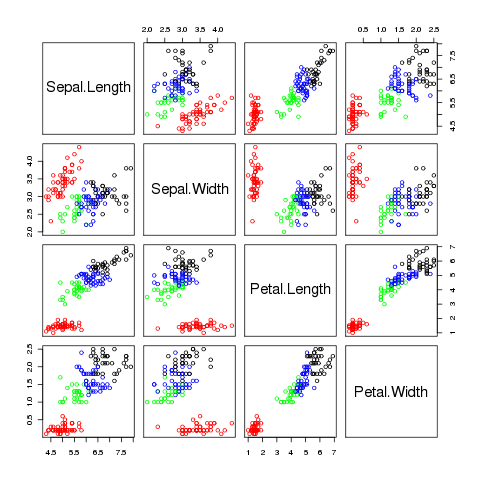
\includegraphics[height = 5.5cm, width = 5.5cm]{plots/plot_exo1_kmeans_2.png}
\includegraphics[height = 5.5cm, width = 5.5cm]{plots/plot_exo1_kmeans_3.png}
\includegraphics[height = 5.5cm, width = 5.5cm]{plots/plot_exo1_kmeans_4.png}
  \caption{Représentation des caractéristiques des données par la méthode des centres mobiles } 
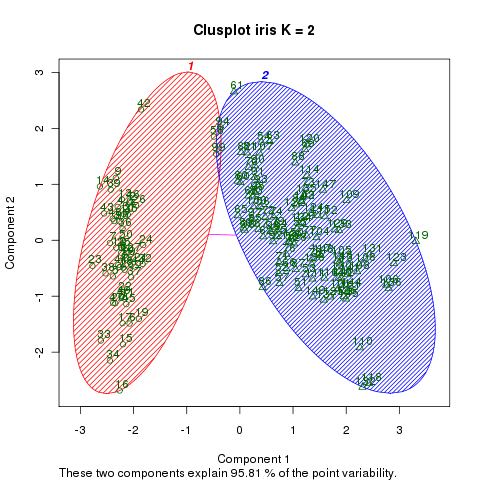
\includegraphics[height = 5.5cm, width = 5.5cm]{plots/clusplot_exo1_kmeans_2.png}
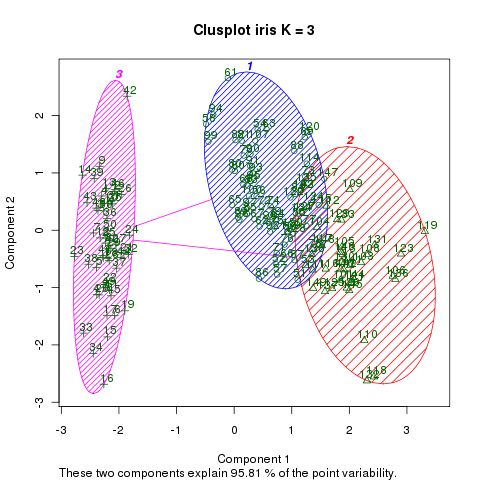
\includegraphics[height = 5.5cm, width = 5.5cm]{plots/clusplot_exo1_kmeans_3.png}
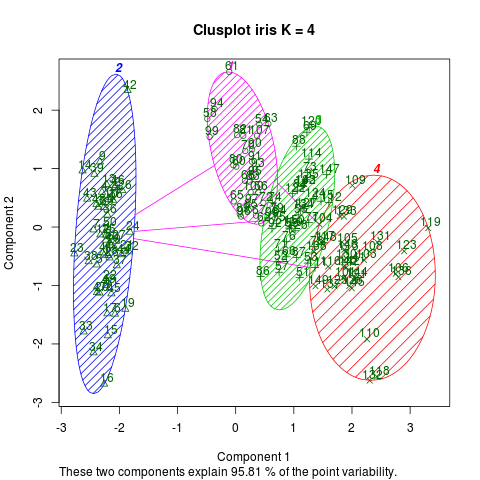
\includegraphics[height = 5.5cm, width = 5.5cm]{plots/clusplot_exo1_kmeans_4.png}
  \caption{Représentation des différentes partitions avec k= 2, 3 et 4 }
\includegraphics[height = 5.5cm, width = 5.5cm]{plots/clusplot_iris_10.png}
\centering
  \caption{Répartition des différentes espèces}
\end{figure}\\
La partition en 2 classes rassemble les espèces Versicolor et Virginica en une seule classe,
ce qui indique que les dissimilarités entre Setosa et les deux autres espèces sont plus importantes qu'entre Virginica et Versicolor.
Il semble donc que l'espèce Setosa soit plus facilement identifiable, contrairement aux deux autres espèces dont les points s'entremêlent.\\ \\
La partition en 3 classes identifie bien les Setosa mais la classification semble moins évidente
pour les points situés à l'intersection des espèces Virginica et Versicolor, puisque de nombreuses erreurs de classification sont commises.
\newpage
\noindent
La partition en 4 classes permet quant à elle de bien identifier les fleurs Setosa et les fleurs qui appartiennent de manière
quasi certaine aux Virginica (classe 4) et Versicolor (classe 2).
La quatrième classe créée (classe 1) semble correspondre aux points d'intersection des Virginica et Versicolor,
où les dissimilarités entre les fleurs de ces espèces sont assez faibles.
Elle permet donc de cibler cette zone d'incertitude où les fleurs peuvent rentrer à la fois dans les critères de Virginica et Versicolor,
ce qui rend la partition en 4 classes particulièrement intéressante par rapport aux deux autres partitions.\\ \\
% QUESTION 1.2
\textbf{Question 2 :}\\
Lors de l'étape initiale de la méthode des kmeans, un nombre de centres initiaux égal
au nombre de classes désirées est pris aléatoirement dans le jeu de données. L’algorithme est ensuite appliqué à ces centres.
Ce mécanisme implique le constat suivant : d’une exécution à l’autre, les points de départ de la méthode ne sont pas les mêmes.\\ \\
Etudier la stabilité du résultat de la partition en 3 classes revient donc à lancer plusieurs fois
d’affilée l’algorithme kmeans (qui aura à chaque fois des centres initiaux différents) et vérifier que les
partitions obtenues sont les mêmes dans tous les cas.\\ \\
Pour cela on utilise l'inertie intra classe, qui décrit l'homogénéité des données à de chaque classe.
Plus les données à l’intérieur d'une classe sont homogènes,
plus les distances des points de la classe par rapport au point représentant la classe sont faibles.
Ainsi, si notre partition est stable, nous devrions retrouver des inerties intra-classe similaires pour chaque classification.\\ \\
Nous avons lancé 100 fois l’algorithme.
Sur les 100 résultats, nous obtenons seulement 2 valeurs différentes,
à savoir 20\% de valeurs égales à 142.75 et 80\% de valeurs 78.85 ce qui signifie que la partition n'est que relativement stable.\\ \\
% QUESTION 1.3
\textbf{Question 3 :}\\
Nous calculons la valeur moyenne d’inertie intraclasse obtenue sur 100 classifications en faisant varier
k entre 2 et 5.
\begin{table}[h]
  \centering
	\begin{tabular}{ccccc}
		Partition &  k = 2 &  k = 3 &  k = 4  &  k = 5 \\
		Moyenne d'inertie intra-classe & 152.348 & 95.46598 & 61.96268 &51.01975\\
	\end{tabular}
  \caption{Moyennes des inerties intra-classe pour les classification avec k = 2, 3, 4, 5}
\end{table}\\
Le graphique suivant permet d’apprécier facilement la valeur de ces moyennes en fonction de k.\\
\begin{figure}[h!]
  \centering
	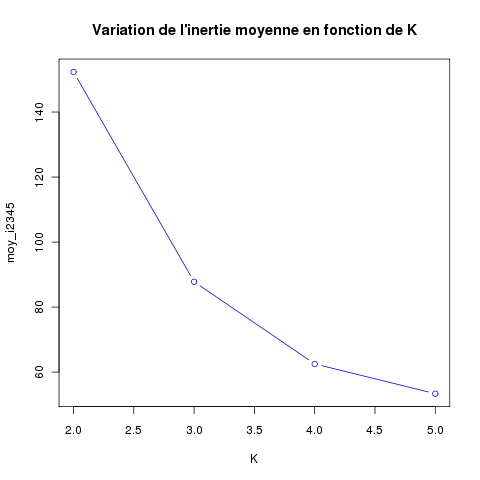
\includegraphics[height = 5cm, width = 7cm]{plots/plot_moy_inerties_k.png}
  \caption{Représentation graphique de l'inertie moyenne en fonction du nombre de classes}
\end{figure}\\
La méthode du coude va nous aider à proposer un nombre optimal de classes pour un jeu de données.
Pour trouver ce nombre de classes optimal, il faut tracer la courbe de l'inertie intra-classe moyenne en fonction du nombre de classes,
puis choisir le nombre de classes correspondant au "coude" de la courbe.\\
On voit ici le "coude" pour un partitionnement en 4 classes.
Cela peut s'expliquer par le fait qu'il y ait cette zone de flou entre 2 classes dans la classification par k = 3,
zone de flou qui est séparée des autres classes dans la classification par k = 4.
\newpage
\noindent
Pour  k = 4, les points d'une même classe sont plus proches de son centre de gravité,
ce qui implique une inertie intra-classe moindre par rapport à k = 3, où les points des classes sont plus étalés.
Les données partitionnées en 4 classes sont donc plus homogènes qu'en 3 classes.
On remarque également que l'inertie intra-classe pour k = 5 ne diffère que de peu de celle pour k = 4.
Un partitionnement en 4 classes semble donc suffisant puisque au-delà le partitionnement ne réduit plus de manière significative l’inertie.\\
Ainsi, bien que la solution k = 4 ne corresponde pas à la distribution initiale qui sépare les données en 3 classes,
ce partitionnement peut être approprié dans notre cas.\\ \\
% QUESTION 1.4
\textbf{Question 4 :}\\
Nous souhaitons comparer la classification obtenue par la méthode des kmeans pour k = 3 avec la classification réelle.
Pour cela nous comptons le nombre de valeurs différentes entre le vecteur réel $donnees\$cls$ et le vecteur $k3\$cluster$ obtenus
grâce à la fonction \texttt{kmeans}. 
Si les fleurs du type Setosa sont identifiées correctement à 100\% par la classe 3,
on remarque 12\% d'erreurs de classification pour Virginica (classe 1) et Versicolor (classe 2),
ce qui correspond certainement à la zone d'intersection observée. 
Nous obtenons donc 92\% de similitude au total entre les deux classifications, un résultat qui n'est donc pas optimal mais reste correct.

\section*{Exercice 2 : Algorithmes EM et CEM}
\subsection*{Données synthétiques}
Dans cette deuxième partie nous étudions les algorithmes EM et CEM dans le cas de données monodimensionnelles,
d'abord avec des données synthétiques puis avec des données réelles.
L'algorithme EM/CEM pour des données monodimensionnelles s'effectue en 3 étapes (resp. 4 pour CEM) :
\begin{enumerate}
\item Initialisation : choix arbitraire d'une solution initiale.
\item Estimation :  pour chaque classe, calcul de la probabilité que les individus des
données lui appartienne.
\item Classification : (seulement dans CEM) classification de chaque individu dans les deux classes \\ (t1 ou t2)
suivant leur probabilité d'appartenance à chaque classe.
\item Maximisation : calcul des nouveaux paramètres $\pi$, $\mu$ et $\sigma^{2}$ en fonction des deux classes t1 et t2 déterminées
lors de l'étape de classification.
\end{enumerate}
% QUESTION 2.1
\textbf{Question 1 :}\\
Les équations de mise à jour des paramètres pour $\mu_{k}$ et $\sigma_{k}$ avec $k \in \{1,2\}$ sont :
\begin{figure}[h!]
  \centering
$\mu^{(c+1)}_{1} = \frac{ \sum_{i} t_{i1}^{(c)}x_{i} }{ \sum_{i} t_{i1}^{(c)} }$ et
$\mu^{(c+1)}_{2} = \frac{ \sum_{i} t_{i2}^{(c)}x_{i} }{ \sum_{i} t_{i2}^{(c)} }$ \\
$(\sigma^{2}_{1})^{(c+1)} = \frac{ \sum_{i} t_{i1}^{(c)}(x_{i}-\mu^{(c+1)}_{1})^{2}}{ \sum_{i} t_{i1}^{(c)} }$ et
$(\sigma^{2}_{2})^{(c+1)} = \frac{ \sum_{i} t_{i2}^{(c)}(x_{i}-\mu^{(c+1)}_{2})^{2}}{ \sum_{i} t_{i2}^{(c)} }$ 
\end{figure}\\ \\
% QUESTION 2.2
\textbf{Question 2 et 3 :}\\
Les résultats observés sont très proches des données théoriques.
\begin{table}[h]
\centering
	\begin{tabular}{cccc}
		 & Valeurs théoriques & EM & CEM\\
		$\mu_{1}$ & 0 & 0.01 & -0.02 \\
		$\mu_{2}$ & 6 & 6.40 &  7.38 \\
		$\sigma_{1}$ & 1 & 1.03 & 1.00 \\
		$\sigma_{2}$ & 5 & 4.99 & 4.59 \\
	\end{tabular}
  \caption{Comparaison des résultats obtenus par l'algorithme EM et l'algorithme CEM par rapport aux valeurs théoriques initiales}
\end{table}\\
On remarque que les valeurs renvoyées par l’algorithme CEM s’écartent plus des valeurs d’origine,
ce qui s’explique par la maximisation à chaque étape de la vraisemblance complétée,
ce qui implique une augmentation de l’écart entre les paramètres.\\
\newpage
\noindent
% QUESTION 2.4
\textbf{Question 4 :}
\begin{figure}[h!]
	\includegraphics[height = 5.5cm, width = 5.5cm]{plots/partition_exo2_kmeans.png}
	\includegraphics[height = 5.5cm, width = 5.5cm]{plots/partition_exo2_EM.png}
	\includegraphics[height = 5.5cm, width = 5.5cm]{plots/partition_exo2_CEM.png}
  \caption{Comparaison des partitions obtenues par les algorithmes kmeans, EM et CEM }
\end{figure}\\
On obtient une première partition des données $x_{i}$ en utilisant l'algorithme \texttt{kmeans},
puis on utilise la fonction \texttt{map()} sur les données générées par les algorithmes EM et CEM afin d'obtenir deux autres partitions
des données $x_{i}$ en 2 classes. Ceci va nous permettre de comparer les partitions effectuées par les trois méthodes sur nos
données théoriques monodimensionnelles.\\
Les graphiques mettent bien en évidence la séparation des deux distributions gaussiennes, de 0 à 1000 pour $\mu_{1}=0$ et $\sigma_{1}=1$,
et de 1000 à 2000 $\mu_{2}=6$ et $\sigma_{2}=5$.\\ \\
La fonction \texttt{randindex} nous fournit des informations complémentaires pour évaluer la similarité entre les partitions.
Les résultats de son exécution son retranscrits dans le tableau ci-dessous.
\begin{table}[h]
\centering
	\begin{tabular}{cccc}
		  & Kmeans & EM & CEM\\
		Kmeans & 1 &  &  \\
		EM & 0.79 &  1 & \\
		CEM & 0.80 & 0.99 &  1\\
	\end{tabular}
  \caption{Comparaison des indices de Rand entre les différentes partitions}
\end{table}\\
On note tout d’abord une grande similarité entre les résultats obtenus par les algorithmes EM
et CEM, ce qi est confirmé par l'idice de Rand qui est de 99\%, avec toutefois un résultat légèrement meilleur avec CEM.
En effet il y'a un peu plus de points qui n'ont pas été partitionnés correctement par l’algorithme EM,
cela se voit notamment dans l'intervalle 0 à 1000, où le graphe EM classe un peu plus de points en rouge (ce qui est faux) que CEM.
C'est donc bien CEM qui a la partition  la plus proche de celle de \texttt{kmeans},
ce qui explique qu'on obtiennent 80\% de similitude entre \texttt{kmeans} et CEM, contre 79\% avec EM.
Pour \texttt{kmeans} comme pour EM/CEM, il y a un certain nombre d’erreurs de classement mais qu'elles ne sont pas de la même nature :
\texttt{kmeans} ne réalise aucune erreur pour la classe 1 (noire) sur l'intervalle 0 à 1000 mais énormément pour les deux classes sur
1000 à 2000, tandis que EM et CEM en font peu sur tout l'intervalle, mais pour les deux classes.\\ \\
L'algorithme \texttt{kmeans} donne un résultat assez différent de ceux obtenus par EM et CEM.
En effet, il semble diviser le nuage de points par une droite horizontale d'équation $x = 5$ :
les $x_{i} > 5$  forment une classe, et les $x_{i} < 5$ en forment une autre.
Les deux classes semblent avoir la même "amplitude" en hauteur, de 15 environ. 
Il semble que l'algorithme \texttt{kmeans} interprète moins bien la structure des données :
en effet, le critère de minimiser la distance entre les centres de gravité et les individus d’une même partition tend à obliger
les points d'une même partition à former un ensemble en un seul bloc et à éviter le plus possible que deux partitions ne s'entrecroisent,
alors que dans notre cas, l’interprétation la plus cohérente implique la séparation de la classe rouge en deux blocs comme
on le remarque sur les deux autres graphes.\\ \\
EM et CEM donnent donc une classification qui semble plus logique, en utilisant deux droites \\ séparatrices :
une classe regroupant les points condensés pour $x$ compris environ entre -2 et 2 et une classe regroupant les points restants.
Les algorithmes EM et CEM arrivent donc à faire une séparation assez correcte d'une classe (noire) dont les points sont entourés par
les points de l'autre classe (rouge).\\
Ainsi, il semble que EM et CEM aient réussi à mieux prendre compte les dispersions des distributions et à comprendre
la structure du jeu de données que \texttt{kmeans}.\\

\subsection*{Données réelles \texttt{crabs}}
On observe que les valeurs des $\mu$ et $\sigma$ sont toutes assez proches de 0,
ce qui implique que les classes définies par ce modèle de mélange sont très proches, voire confondables.\\
\begin{table}[h]
\centering
	\begin{tabular}{cc}
		  & EM \\
		$\mu_{1}$ & 0.39 \\
		$\mu_{2}$ & 0.88\\
		$\sigma_{1}$ & 0.04 \\
		$\sigma_{2}$ & 0.02  \\
	\end{tabular}
  \caption{Résultat obtenu par l'algorithme EM  pour un modèle de mélange à 2 composantes}
\end{table}\\
Aussi lorsque l’on essaie de partitionner les données en 2 classes en ne s’appuyant que sur une
seule variable à la fois, nous observons que toutes les données sont classées dans une seule et même classe.
On en déduit que la méthode mono-dimensionnelle n’est pas suffisante pour un tel jeu de
données, et qu’il faut donc les traiter de manière multidimensionnelle.\\
\begin{figure}[h!]
\centering
	\includegraphics[height = 7cm, width = 7cm]{plots/partition_exo2_crabs1.png}
	\includegraphics[height = 7cm, width = 7cm]{plots/partition_exo2_crabs2.png}
  \caption{Comparaison des classifications des données à partir de la première et de la deuxième variable}
\end{figure}\\ \\

\section*{Exercice 3 : Mélange gaussien multidimensionnel}
\subsection*{Données synthétiques}
% QUESTION 3.1
\textbf{Question 1 :}\\
La fonction densité d'un mélange gaussien multidimensionnel est de la forme :\\
$f(x_{i}; \theta) = \underset{k}{\sum} \pi_{k} \varphi (x_{i}; \mu_{k}, \Sigma_{k})$ avec 
$\theta = (\pi_{1}, \pi_{2}, \pi_{3}, \mu_{1}, \mu_{2}, \mu_{3}, \Sigma_{1}, \Sigma_{2}, \Sigma_{3})$.\\
La densité conditionnelle de la loi normale multidimensionnelle vaut :\\
$\varphi(x; \mu_{k}, \Sigma_{k}) = \frac{1}{(2 \pi)^{\frac{p}{2}}|\Sigma_{k}|^\frac{1}{2}}
exp\{-\frac{1}{2} (x - \mu_{k})' \Sigma_{k}^{-1} (x - \mu_{k})\}$ \\
Le modèle de classes latentes suppose que les variables sont conditionnellement indépendantes connaissant la classe.\\
La partition ou matrice de classification $c = (c_{ik})$, avec $c_{ik} = t_{ik}$ pour l'algorithme EM et
la partition $c = (c_{ik})$ avec $c_{ik} = z_{ik}$ pour l'algorithme CEM, sert à unifier la présentation.\\
Le cardinal $n_{k}$ de la classe $k$ : $n_{k} = \sum_{i} c_{ik}$.
\newpage
\noindent
La maximisation en $\theta$ s'écrit dans le cas gaussien multidimensionnel :\\
$-\frac{1}{2} \underset{i, k}{\sum} c_{ik} (x_{i} - \mu_{k})' \Sigma_{k}^{-1} (x_{i} - \mu_{k})
- \frac{1}{2} \underset{k}{\sum} n_{k} log|\Sigma_{k}| + \underset{k}{\sum} n_{k} log \pi_{k}$\\ \\
La maximisation de $\underset{k}{\sum} n_{k} log \pi_{k}$ nous donne la proportion $\pi_{k} = \frac{n_{k}}{n}$.\\
La maximisation de $-\frac{1}{2} \sum_{i,k} c_{ik} (x_{i} - \mu_{k})' \Sigma_{k}^{-1} (x_{i} - \mu_{k})$ nous donne la moyenne
$\mu_{k} = \frac{1}{n_{k}} \underset{i}{\sum} c_{ik} x_{i}$.\\
Les $\Sigma_{k}$ doivent minimiser la fonction $F(\Sigma_{1}, \Sigma_{2}, \Sigma_{3}) =
\underset{k}{\sum} n_{k} (trace(S_{k} \Sigma_{k}^{-1}) + log|\Sigma_{k}|)$,
ce qui nous donne la matrice de variance de la classe k : 
$\Sigma_{k} = S_{k} = \frac{1}{n_{k}} \sum_{i} c_{ik} (x_{i} - \mu_{k}) (x_{i} - \mu_{k})'$.\\ \\
% QUESTION 3.2
\textbf{Question 2 :}\\
Concernant l'implémentation des algorithmes EM et CEM, nous avons rencontré un problème sur le $\Sigma_{k}$ puisque
le calcul de la densité conditionnelle
$\varphi(x_{i}; \mu_{k}, \Sigma_{k})$ qui contenait un calcul du déterminant de $\Sigma_{k}$ nous retournait des valeurs infinies.
Nous n'avons pas été en mesure de déterminer et de corriger notre erreur dans l'implémentation de ces algorithmes.\\ \\
% QUESTION 3.3
\textbf{Question 3 :}\\
L'application de la méthode des $kmeans$ nous donne le graphique suivant :\\
\includegraphics[height = 7cm, width = 7cm]{plots/plot_exo3_kmeans_3.png}\\
L'étude de ce graphique issu de la méthode des $kmeans$ nous permet d'observer clairement les 3 classes de données que nous avons utilisé au
début.\\ \\

\subsection*{Application aux données réelles}
L'application de la méthode des $kmeans$ sur les données réelles nous donne le graphique suivant :\\
\includegraphics[height = 7cm, width = 7cm]{plots/plot_exo3_kmeans_4.png}\\
Nous pouvons remarquer sur ce graphique que les 2 espèces de crabs sont plutôt bien identifiées,
ainsi que les classes regroupant les crabes selon le sexe et l'espèce.\\ \\

  \end{document}
